\documentclass[letterpaper,12pt,fleqn]{article}
\usepackage{matharticle}
\pagestyle{empty}
\newcommand{\e}{\epsilon}
\renewcommand{\d}{\delta}
\begin{document}
\section*{Limits}

\begin{definition}
  To say that:
  \[\lim_{z\to z_0}f(z)=L\]
  means:
  \[\forall\,\e>0,\exists\,\d>0,0<\abs{z-z_0}<\d\implies\abs{f(z)-L}<\e\]
\end{definition}

For all $z$ in an arbitrarily small deleted neighborhood for $z_0$, there
exists an image in the arbitrarily small neighborhood for $w_0$.

\begin{minipage}[t]{3in}
  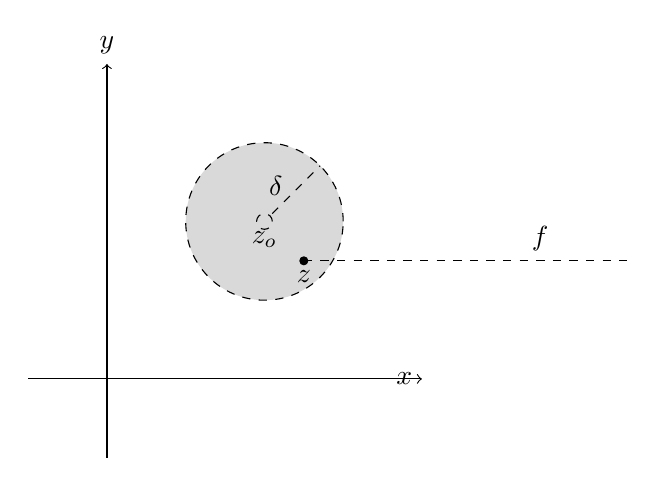
\begin{tikzpicture}
    \draw [->] (-1,0) -- (4,0);
    \draw [->] (0,-1) -- (0,4);
    \node [left] at (4,0) {$x$};
    \node [above] at (0,4) {$y$};
    \draw [dashed,fill=gray!30] (2,2) circle [radius=1];
    \draw [dashed] (2,2) circle [radius=0.1];
    \node [below] at (2,2) {$z_o$};
    \draw [dashed] (2.1,2.1) -- ({2+cos(45)},{2+sin(45)});
    \node [left] at ({2+0.5*cos(45)},{2.1+0.5*sin(45)}) {$\d$};
    \draw [fill=black] (2.5,1.5) circle [radius=0.05];
    \node [below] at (2.5,1.5) {$z$};
    
    \draw [dashed] (2.5,1.5) -- (6.6,1.5);
    \node [above] at (5.5,1.5) {$f$};
  \end{tikzpicture}
\end{minipage}
\begin{minipage}[t]{3in}
  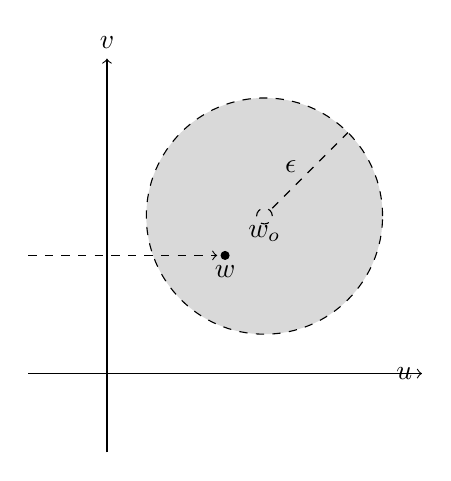
\begin{tikzpicture}
    \draw [->] (-1,0) -- (4,0);
    \draw [->] (0,-1) -- (0,4);
    \node [left] at (4,0) {$u$};
    \node [above] at (0,4) {$v$};
    \draw [dashed,fill=gray!30] (2,2) circle [radius=1.5];
    \draw [dashed] (2,2) circle [radius=0.1];
    \node [below] at (2,2) {$w_o$};
    \draw [dashed] (2.1,2.1) -- ({2+1.5*cos(45)},{2+1.5*sin(45)});
    \node [left] at ({2+0.75*cos(45)},{2.1+0.75*sin(45)}) {$\e$};
    \draw [fill=black] (1.5,1.5) circle [radius=0.05];
    \node [below] at (1.5,1.5) {$w$};

    \draw [dashed,->] (-1,1.5) -- (1.4,1.5);
  \end{tikzpicture}
\end{minipage}

\begin{example}
  Prove:
  \[\lim_{z\to i}\frac{iz}{3}=-\frac{1}{3}\]

  \begin{minipage}[t]{3in}
    Assume $\e>0$ \\
    Let $\d=3\e>0$ \\
    Assume $0<\abs{z-i}<\d$
    
    \begin{eqnarray*}
      \abs{\frac{iz}{3}+\frac{1}{3}} &=&
      \abs{\frac{i}{3}\left(z-i\right)} \\
      &=& \abs{\frac{1}{3}}\abs{z-i} \\
      &<& \frac{\d}{3} \\
      &=& \e \\
    \end{eqnarray*}
  \end{minipage}
  \begin{minipage}[t]{3in}
    \begin{eqnarray*}
      \abs{\frac{iz}{3}+\frac{1}{3}} &=&
      \abs{\frac{i}{3}\left(z-i\right)} \\
      &=& \abs{\frac{1}{3}}\abs{z-i} \\
      &<& \frac{\d}{3} \\
      \e &=& \frac{\d}{3} \\
      \d &=& 3\e \\
    \end{eqnarray*}
  \end{minipage}
\end{example}

\begin{example}
  Prove:
  \[\lim_{z\to z_0}z^2=z_0^2\]

  \begin{minipage}[t]{3.5in}
    Assume $\e>0$ \\
    Let $\d=\sqrt{\e+\abs{z_0}^2}-\abs{z_0}>0$ \\
    Assume $0<\abs{z-z_0}<\d$
    
    \begin{eqnarray*}
      \abs{z^2-z_0^2} &=& \abs{(z-z_0)(z+z_0)} \\
      &=& \abs{z-z_0}\abs{z+z_0} \\
      &=& \abs{z-z_0}\abs{z-z_0+2z_0} \\
      &<& \d\abs{\d+2z_o} \\
      &=& \d^2+2z_0\d \\
      &=& (\d^2+2z_0\d+\abs{z_0}^2)-\abs{z_0}^2 \\
      &=& (\d+\abs{z_0})^2-\abs{z_0}^2 \\
      &=& \left[\left(\sqrt{\e+\abs{z_0}^2}-\abs{z_0}\right)+\abs{z_0}\right]^2-
      \abs{z_0}^2 \\
      &=& \left(\sqrt{\e+\abs{z_0}^2}\right)^2-\abs{z_0}^2 \\
      &=& \e+\abs{z_0}^2-\abs{z_0}^2 \\
      &=& \e \\
    \end{eqnarray*}
  \end{minipage}
  \begin{minipage}[t]{3in}
    \begin{eqnarray*}
      \abs{z^2-z_0^2} &=& \abs{(z-z_0)(z+z_0)} \\
      &=& \abs{z-z_0}\abs{z+z_0} \\
      &=& \abs{z-z_0}\abs{z-z_0+2z_0} \\
      &<& \d\abs{\d+2z_o} \\
      &=& \d^2+2z_0\d \\
      &=& (\d^2+2z_0\d+\abs{z_0}^2)-\abs{z_0}^2 \\
      &=& (\d+\abs{z_0})^2-\abs{z_0}^2 \\
      \e &=& (\d+\abs{z_0})^2-\abs{z_0}^2 \\
      (\d+\abs{z_0})^2 &=& \e+\abs{z_0}^2 \\
      \d+\abs{z_0} &=& \sqrt{\e+\abs{z_0}^2} \\
      \d &=& \sqrt{\e+\abs{z_0}^2}-\abs{z_0} \\
    \end{eqnarray*}
  \end{minipage}
\end{example}

\begin{example}
  Prove:
  \[\lim_{z\to z_0}Re(z)=Re(z_0)\]

  \begin{minipage}[t]{3in}
    Assume $\e>0$ \\
    Let $\d=\e$ \\
    Assume $0<\abs{z-z_0}<\d$
    
    \begin{eqnarray*}
      \abs{Re(z)-Re(z_0)} &=& \abs{Re(z-z_0)} \\
        &\le& \abs{z-z_0} \\
        &<& \d \\
        &=& \e \\
    \end{eqnarray*}
  \end{minipage}
  \begin{minipage}[t]{3in}
    \begin{eqnarray*}
      \abs{Re(z)-Re(z_0)} &=& \abs{Re(z-z_0)} \\
        &\le& \abs{z-z_0} \\
        &<& \d \\
        \e &=& \d \\
    \end{eqnarray*}
  \end{minipage}
\end{example}
\newpage
\begin{example}
  Let $z=x+iy$. Prove:
  \[\lim_{z\to 1-i}[x+i(2x+y)]=1+i\]

  $x+i(2x+y)=(x+iy)+i2x=z+i2Re(z)$

  WTS: $\lim_{z\to z_0}[z+i2Re(z)]=z_0+i2Re(z_0)$
  \begin{eqnarray*}
    \abs{[z+i2Re(z)]-[z_0+i2Re(z_0)]} &=& \abs{(z-z_0)+2i[Re(z)-Re(z_0)]} \\
    &=& \abs{(z-z_0)+2i[Re(z-z_0)]} \\
    &\le& \abs{(z-z_0)}+\abs{2iRe(z-z_0)} \\
    &\le& \abs{z-z_0}+2\abs{z-z_0} \\
    &=& 3\abs{z-z_0} \\
    &=& 3\d \\
    \e &=& 3\d \\
    \d &=& \frac{\e}{3} \\
  \end{eqnarray*}

  Assume $\e>0$ \\
  Let $\d=\frac{\e}{3}$ \\
  Assume $0<\abs{z-z_0}<\d$
  \begin{eqnarray*}
    \abs{[z+2iRe(z)]-[z_0+2iRe(z_0)]} &=& \abs{(z-z_0)+2i[Re(z)-Re(z_0)]} \\
    &=& \abs{(z-z_0)+2iRe(z-z_0)} \\
    &\le& \abs{(z-z_0)}+\abs{2iRe(z-z_0)} \\
    &\le& \abs{z-z_0}+2\abs{z-z_0} \\
    &=& 3\abs{z-z_0} \\
    &<& 3\d \\
    &=& 3\left(\frac{\e}{3}\right) \\
    &=& \e \\
  \end{eqnarray*}

  \begin{eqnarray*}
    \lim_{z\to 1-i}[x+i(2x+y)]=1+i &=& \lim_{z\to 1-i}[z+i2Re(z)] \\
    &=& (1-i)+i2Re(1-i) \\
    &=& 1-i+2i \\
    &=& 1+i \\
  \end{eqnarray*}  
\end{example}
\newpage
\begin{theorem}
$\lim_{z\to z_0}f(z)$ exists $\implies$ the limit is unique.
\end{theorem}

\begin{theproof}
  Assume $\lim_{z\to z_0}f(z)$ exists \\
  Assume $\lim_{z\to z_0}f(z)=w_0$ and $\lim_{z\to z_0}f(z)=w_1$ \\
  Assume $\e>0$ \\
  $\exists\,\d_0>0,0<\abs{z-z_0}<\d_0\implies\abs{f(z)-w_0}<\frac{\e}{2}$ \\
  $\exists\,\d_1>0,0<\abs{z-z_0}<\d_1\implies\abs{f(z)-w_1}<\frac{\e}{2}$ \\
  Let $\d=\min\{\d_0,\d_1\}$ \\
  Assume $0<\abs{z-z_0}<\d$ \\
  \begin{eqnarray*}
    \abs{w_0-w_1} &=& \abs{w_0-f(z)+f(z)-w_1} \\
    &le& \abs{w_0-f(z)}+\abs{f(z)-w_1} \\
    &=& \abs{f(z)-w_0}+\abs{f(z)-w_1} \\
    &<& \frac{\e}{2}+\frac{\e}{2} \\
    &=& \e \\
  \end{eqnarray*}
  $w_0-w_1=0$ \\
  $\therefore w_0=w_1$
\end{theproof}

\begin{corollary}
  If a limit is not unique then it does not exist.
\end{corollary}

\begin{example}
  Prove that the following limit does not exist:
  \[\lim_{z\to0}\frac{\bar{z}}{z}\]

  Path along postive real axis:

  $z=x$ \\
  $\bar{z}=x$ \\
  $\lim_{z\to0}\frac{\bar{z}}{z}=\lim_{z\to0}\frac{x}{x}=1$

  Path along postive imaginary axis:

  $z=iy$ \\
  $\bar{z}=-iy$ \\
  $\lim_{z\to0}\frac{\bar{z}}{z}=\lim_{z\to0}\frac{-iy}{iy}=-1$

  The limits differ based on path \\
  $\therefore$ the limit DNE.
\end{example}

\end{document}
